\documentclass[letter,12pt]{article}
\usepackage[paperheight=27.94cm,paperwidth=21.59cm,bindingoffset=0in,left=3cm,right=2.0cm, top=3.5cm,bottom=2.5cm, headheight=200pt, headsep=1.0\baselineskip]{geometry}
\usepackage{graphicx,lastpage}
\usepackage{upgreek}
\usepackage{censor}
\usepackage[spanish,es-tabla]{babel}
\usepackage{pdfpages}
\usepackage{tabularx}
\usepackage{graphicx}
\usepackage{adjustbox}
\usepackage{xcolor}
\usepackage{colortbl}
\usepackage{rotating}
\usepackage{multirow}
\usepackage[utf8]{inputenc}
\usepackage{float}
\usepackage{hyperref}
\usepackage{minted}

\renewcommand{\tablename}{Tabla}
\usepackage{fancyhdr}
\pagestyle{fancy}

\fancyhead[L]{}
%
\begin{document}
%
   \title{\Huge{Informe Laboratorio 3}}

   \author{\textbf{Sección 3} \\  \\Ihan San Martin \\ e-mail: ihan.sanmartin@mail.udp.cl}
          
   \date{\today}

   \maketitle
   
   \tableofcontents
 
  \newpage
  

\section{Descripción de actividades}
Su objetivo será auditar la implementación de algoritmos hash aplicados a contraseñas en páginas web desde el lado del cliente, así como evaluar la efectividad de estas medidas contra ataques de tipo Pass the Hash (PtH). Para llevar a cabo esta auditoría, deberá registrarse en un sitio web y crear una cuenta, ingresando una contraseña específica para realizar las pruebas.\par

Al concluir la tarea, es importante que modifique su contraseña por una diferente para garantizar su seguridad.\par

Dado que la cantidad de sitios chilenos que utilizan hash es limitada, se permite realizar esta tarea en cualquier sitio web a nivel mundial. En este sentido, realice las siguientes actividades:


\begin{itemize}
    \item Identificación del algoritmo de hash utilizado para las contraseñas al momento del registro en el sitio.
    
    \item Identificación del algoritmo de hash utilizado para las contraseñas al momento de iniciar sesión.

    \item Generación del hash de la contraseña desde la consola del navegador, partiendo de la contraseña en texto plano.

    \item Interceptación del tráfico de login utilizando BurpSuite desde su equipo.

    \item Realización de un intento de login, modificando una contraseña incorrecta por el hash obtenido en el punto anterior.

    \item Descripción de las políticas de privacidad o seguridad relacionadas con las contraseñas, incluyendo un enlace a las mismas.

    \item Cuatro conclusiones sobre la seguridad o vulnerabilidad de la implementación observada.
    


    
\end{itemize}

\newpage
\section{Desarrollo de actividades según criterio de rúbrica}

Para el desarrollo de esta experiencia de laboratorio se utilizó la página web \textbf{\textit{mega.io \slash mega.nz}}, con un poco de investigación se descubrió que este servicio de almacenamiento en la nube y file-sharing hace \textbf{hashing} en el lado del cliente, esto debido a su mecanismo de \textbf{zero-knowledge}, que básicamente significa que toda la encriptación y desencriptación se hace en el dispositivo del usuario, de esa forma ni siquiera MEGA puede acceder a tus archivos y obviamente la contraseña en texto plano.

\begin{figure}[H]
    \centering
    
\includegraphics[width=0.75\linewidth]{mega.png}
    \caption{Logotipo de mega.io/mega.nz}
\end{figure}

Antes de comenzar con cada punto de la rúbrica, se debe empezar por crear una cuenta, monitoreando las peticiones \textbf{HTTP} que se hacen para analizar qué sucede internamente en la página. Para esta prueba se utilizó un correo electrónico personal con la contraseña ``@criptoyseg''. Se hacen variadas peticiones del tipo \textbf{POST}, pero la más importante fue la siguiente.

\begin{figure}[H]
    \centering
    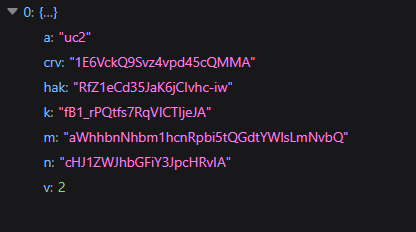
\includegraphics[width=0.6\linewidth]{peticionHak.png}
    \caption{Petición de registro con datos encriptados}
\end{figure}

Esta contiene distintas cadenas que se derivan de la contraseña, correo, un salt generado aleatoriamente, etc.

\subsection{Identifica el algoritmo de hash utilizado al momento de registrarse en el sitio}

Para identificar el algoritmo utilizado, hizo falta entrar en los archivos de la página, específicamente al script que maneja el inicio de sesión y registro de cuentas. Específicamente se analizó un script sin nombre fijo que va variando por cada vez que se recarga la página, es del tipo ``0c09f628-6b90-4875-99c0-d1002144fee7''.

Para acceder por cuenta propia a los archivos de la página se siguieron los siguientes pasos con el navegador Firefox:
\begin{itemize}
    \item F12 $>$ Debugger $>$ Main Thread $>$ blob:// $>$ https://mega.nz $>$ [SCRIPT]
\end{itemize}

Lo primero que se buscó fue la función que maneja el registro de usuarios y se encontró el siguiente bloque de código.

\begin{minted}[linenos, breaklines, highlightlines={29}, highlightcolor=yellow!30]{javascript}
startRegistration: function(firstName, lastName, email, password, fromProPage, completeCallback, skipLoading) {
        'use strict';

        if (this.sendEmailRequestParams) {
            console.error('startRegistration blocked, ongoing.');
            return;
        }
        this.sendEmailRequestParams = true;

        if (!skipLoading) {
            // Show loading dialog
            loadingDialog.show();
        }

        // First create an ephemeral account and the Master Key (to be removed at a later date)
        security.register.createEphemeralAccount(function() {

            // Derive the Client Random Value, Encrypted Master Key and Hashed Authentication Key
            security.deriveKeysFromPassword(password, u_k)
                .then(({clientRandomValueBytes, encryptedMasterKeyArray32, hashedAuthenticationKeyBytes}) => {

                    // Encode parameters to Base64 before sending to the API
                    const req = {
                        a: 'uc2',
                        n: base64urlencode(to8(firstName + ' ' + lastName)),         // Name (used just for the email)
                        m: base64urlencode(email),                                   // Email
                        crv: ab_to_base64(clientRandomValueBytes),                   // Client Random Value
                        k: a32_to_base64(encryptedMasterKeyArray32),                 // Encrypted Master Key
                        hak: ab_to_base64(hashedAuthenticationKeyBytes),             // Hashed Authentication Key
                        v: 2                                                         // Version of this protocol
                    };

                    // If this was a registration from the Pro page
                    if (fromProPage === true) {
                        req.p = 1;
                    }

                    // Send signup link email
                    security.register.sendSignupLink(req, firstName, lastName, email, completeCallback);
                });
        });
    }
\end{minted}

Este bloque nos da la pista de donde viene el campo hak (linea 29) de la petición POST que se encontró, ya que esta función se encarga de construir la petición con todos los campos necesarios, así que luego de esto se va buscando inversamente cómo se construye la variable \textbf{hashedAuthenticationKeyBytes}.

Buscando en el código se encontró el siguiente bloque de la función \textbf{deriveKeysFromPassword}.

\begin{minted}[linenos, breaklines, highlightlines={8, 15, 19, 26}, highlightcolor=yellow!30]{javascript}

    deriveKeysFromPassword: async function(password, masterKeyArray32) {
        'use strict';

        // Create the 128 bit (16 byte) Client Random Value and Salt
        var saltLengthInBytes = security.saltLengthInBits / 8;
        var clientRandomValueBytes = crypto.getRandomValues(new Uint8Array(saltLengthInBytes));
        var saltBytes = security.createSalt(clientRandomValueBytes);

        // Trim the password and convert it from ASCII/UTF-8 to a byte array
        var passwordTrimmed = $.trim(password);
        var passwordBytes = security.stringToByteArray(passwordTrimmed);

        // The number of iterations for the PPF and desired length in bits of the derived key
        var iterations = security.numOfIterations;
        var derivedKeyLength = security.derivedKeyLengthInBits;

        // Run the PPF
        const derivedKeyBytes = await security.deriveKey(saltBytes, passwordBytes, iterations, derivedKeyLength);

        // Get the first 16 bytes as the Encryption Key and the next 16 bytes as the Authentication Key
        const derivedEncryptionKeyBytes = derivedKeyBytes.subarray(0, 16);
        const derivedAuthenticationKeyBytes = derivedKeyBytes.subarray(16, 32);

        // Get a hash of the Authentication Key which the API will use for authentication at login time
        let hashedAuthenticationKeyBytes = asmCrypto.SHA256.bytes(derivedAuthenticationKeyBytes);

        // Keep only the first 128 bits (16 bytes) of the Hashed Authentication Key
        hashedAuthenticationKeyBytes = hashedAuthenticationKeyBytes.subarray(0, 16);

        // Convert the Derived Encryption Key to a big endian array of 32 bytes, then encrypt the Master Key
        const derivedEncryptionKeyArray32 = base64_to_a32(ab_to_base64(derivedEncryptionKeyBytes));
        const cipherObject = new sjcl.cipher.aes(derivedEncryptionKeyArray32);
        const encryptedMasterKeyArray32 = encrypt_key(cipherObject, masterKeyArray32);

        // Pass the Client Random Value, Encrypted Master Key and Hashed Authentication Key to the calling function
        return {
            clientRandomValueBytes,
            encryptedMasterKeyArray32,
            hashedAuthenticationKeyBytes,
            derivedAuthenticationKeyBytes
        };
    }
    
\end{minted}

Esta función se encarga de calcular cada valor de los campos de la petición POST, el que nos interesa es el hak (hashed authentication key) y como se puede ver en la linea 26 del bloque anterior, hashedAuthenticationKeyBytes se calcula con el hash SHA-256. Pero esto no es todo, también en la linea 19, se puede ver como se usa la función \textbf{deriveKey}, con varios parámetros importantes, como el salt, la contraseña, el número de iteraciones que se define en otra parte del código como 100.000, y un largo de bits, entonces investigando más en el código se encontraron las funciones ``Padre'' de la encriptación de esta página.

\begin{minted}[linenos, breaklines, highlightlines={29-34, 61}, highlightcolor=yellow!30]{javascript}

    deriveKey: async function(saltBytes, passwordBytes, iterations, derivedKeyLength) {
        'use strict';

        // If Web Crypto method supported, use that as it's nearly as fast as native
        if (window.crypto && window.crypto.subtle && !window.is_microsoft) {
            return security.deriveKeyWithWebCrypto(saltBytes, passwordBytes, iterations, derivedKeyLength);
        }

        // Otherwise, use asmCrypto which is the next fastest
        return security.deriveKeyWithAsmCrypto(saltBytes, passwordBytes, iterations, derivedKeyLength);
    },

    /**
     * Derive the key using the Web Crypto API
     * @param {Uint8Array} saltBytes The salt as a byte array
     * @param {Uint8Array} passwordBytes The password as a byte array
     * @param {Number} iterations The cost factor / number of iterations of the PPF to perform
     * @param {Number} derivedKeyLength The length of the derived key to create
     */
    deriveKeyWithWebCrypto: async function(saltBytes, passwordBytes, iterations, derivedKeyLength) {
        'use strict';

        // Import the password as the key
        return crypto.subtle.importKey('raw', passwordBytes, 'PBKDF2', false, ['deriveBits'])
            .then((key) => {

                // Required PBKDF2 parameters
                var params = {
                    name: 'PBKDF2',
                    hash: 'SHA-512',
                    salt: saltBytes,
                    iterations: iterations
                };

                // Derive bits using the algorithm
                return crypto.subtle.deriveBits(params, key, derivedKeyLength);
            })
            .then((derivedKeyArrayBuffer) => {

                // Convert to a byte array
                // Pass the derived key to the callback
                return new Uint8Array(derivedKeyArrayBuffer);
            });
    },

    /**
     * Derive the key using asmCrypto
     * @param {Uint8Array} saltBytes The salt as a byte array
     * @param {Uint8Array} passwordBytes The password as a byte array
     * @param {Number} iterations The cost factor / number of iterations of the PPF to perform
     * @param {Number} derivedKeyLength The length of the derived key to create
     */
    deriveKeyWithAsmCrypto: async function(saltBytes, passwordBytes, iterations, derivedKeyLength) {
        'use strict';

        // Convert the desired derived key length to bytes and derive the key
        var keyLengthBytes = derivedKeyLength / 8;

        // Pass the derived key to the callback
        return asmCrypto.PBKDF2_HMAC_SHA512.bytes(passwordBytes, saltBytes, iterations, keyLengthBytes);
    }
    
\end{minted}

Como se puede observar en el bloque de código, las funciones deriveKeyWithWebCrypto y deriveKeyWithAsmCrypto utilizan el algoritmo PBKDF2 con HMAC-SHA512, que es un algoritmo de derivación de claves que aplica múltiples iteraciones de hashing para aumentar la seguridad de las contraseñas. En este caso, se utiliza un salt generado aleatoriamente y 100.000 iteraciones, lo que hace que el proceso de hashing sea más lento y resistente a ataques de fuerza bruta.

Este conjunto de funciones calculan la clave derivada maestra de 32 bytes, la cual se divide a la mitad, y es sólo una mitad a la cual se le aplica un hash SHA-256 para generar el parámetro hak.

\subsection{Identifica el algoritmo de hash utilizado al momento de iniciar sesión}

Para el caso del login el flujo es un poco distinto, y se puede evidenciar en el siguiente bloque de código, que es la función que maneja el inicio de sesión.

\begin{minted}[linenos, breaklines, highlightlines={32-38}, highlightcolor=yellow!30]{javascript}
    
    startLogin: function(email, password, pinCode, rememberMe, salt, loginCompleteCallback) {

        'use strict';

        // Convert the salt and password to byte arrays
        var saltArrayBuffer = base64_to_ab(salt);
        var saltBytes = new Uint8Array(saltArrayBuffer);
        var passwordBytes = security.stringToByteArray(password);

        // The number of iterations for the PPF and desired length in bits of the derived key
        var iterations = security.numOfIterations;
        var derivedKeyLength = security.derivedKeyLengthInBits;

        // Set the callback to run after login is complete
        security.login.loginCompleteCallback = loginCompleteCallback;

        // Store the remember-me flag for any direct cals to this function (e.g. atomicSignIn)
        security.login.rememberMe = rememberMe !== false;

        // Run the PPF
        return security.deriveKey(saltBytes, passwordBytes, iterations, derivedKeyLength).then((derivedKeyBytes) => {

            // Get the first 16 bytes as the Encryption Key and the next 16 bytes as the Authentication Key
            var derivedEncryptionKeyBytes = derivedKeyBytes.subarray(0, 16);
            var derivedAuthenticationKeyBytes = derivedKeyBytes.subarray(16, 32);
            var authenticationKeyBase64 = ab_to_base64(derivedAuthenticationKeyBytes);

            // Convert the Derived Encryption Key to a big endian array of 32 bit values for decrypting the Master Key
            var derivedEncryptionKeyArray32 = base64_to_a32(ab_to_base64(derivedEncryptionKeyBytes));

            // Authenticate with the API
            return security.login.sendAuthenticationKey(
                email,
                pinCode,
                authenticationKeyBase64,
                derivedEncryptionKeyArray32
            );
        }).catch((ex) => {
            // @todo revamp and ditch the callbacks hell... {ref: atomicSignIn}
            if (security.login.loginCompleteCallback) {
                return security.login.loginCompleteCallback(ex);
            }
            throw ex;
        });
    }

\end{minted}

En las lineas 32 a 38 se puede observar que la authenticación se hace a través de la API, esto significa que ya no es del lado del cliente como en el registro, pero para verificar el acceso se deben usar los mismo algoritmos que para el registro para obtener el hash y compararlo con el que se encuentra guardado en la base de datos, es decir se utiliza PBKDF2 con HMAC-SHA512 y SHA-256.

\subsection{Genera el hash de la contraseña desde la consola del navegador}

Para comprobar el funcionamiento del hashing por lado del cliente, se puede generar el hash de la contraseña desde la consola del navegador utilizando el siguiente código:

\begin{figure}[H]
    \centering
    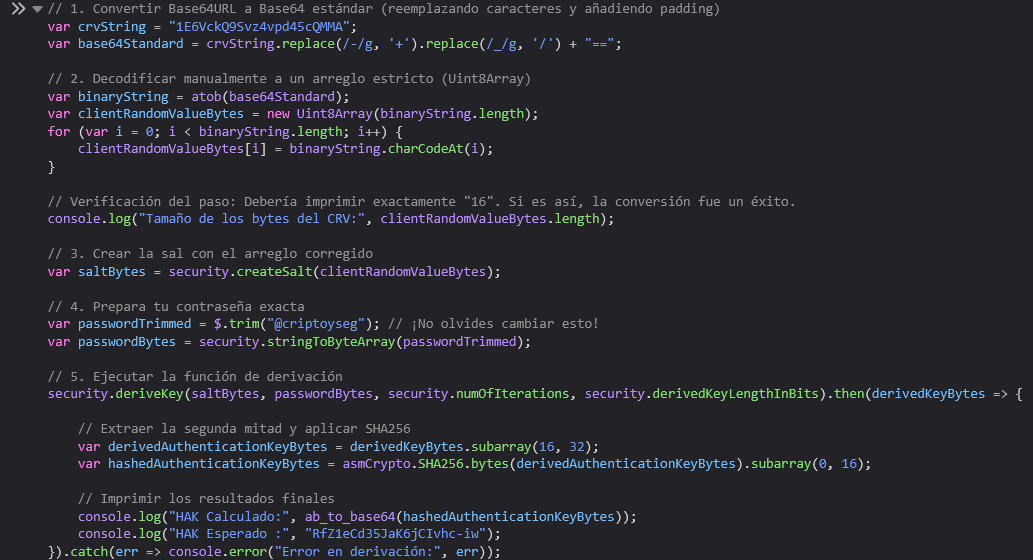
\includegraphics[width=0.9\textwidth]{codigoConsola.png}
    \caption{Código para generar el hash de la contraseña en la consola del navegador}
\end{figure}

Primero se necesita saber los valores de la petición por dos razones:
\begin{itemize}
    \item Obtener el salt exacto del usuario que es necesario para el hash final.
    \item Saber cuál es el valor de hak para comparar el resultado calculado en la consola, con el hak real del usuario.
\end{itemize}

Luego se debe modificar el campo de la contraseña en el código con la que usamos de prueba, que en este caso fue ``@criptoyseg'' y finalmente al ejecutar el código, se obtuvo el siguiente resultado.

\begin{figure}[H]
    \centering
    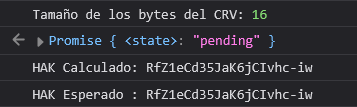
\includegraphics[width=0.9\textwidth]{resultadoConsola.png}
    \caption{Resultado de la generación del hash de la contraseña en la consola del navegador}
\end{figure}

El hak esperado es el mismo valor que se observa en la figura 2, y el calculado coincide, así completando el objetivo de este punto.

\subsection{Intercepta el tráfico login con BurpSuite}

Al igual que se hizo en el laboratorio número 2, se utilizó BurpSuite para interceptar el tráfico con su función proxy y su navegador interno. En la figura 5 se puede ver el formulario de login de MEGA con los datos utilizados de prueba.

\begin{figure}[H]
    \centering
    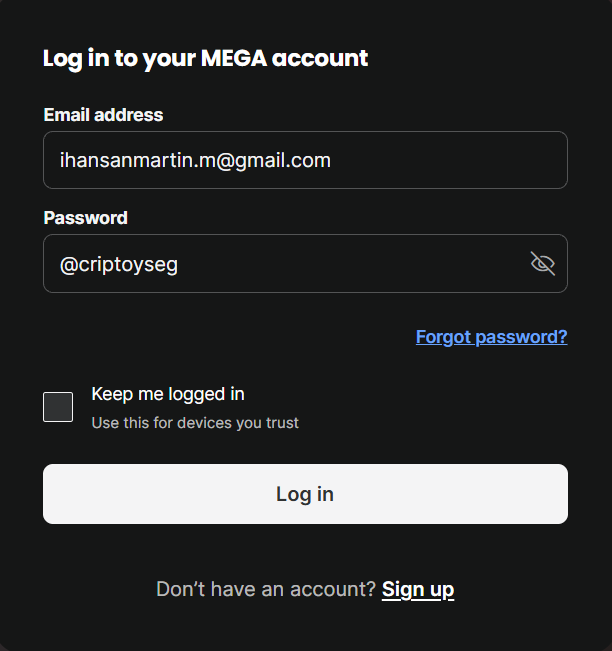
\includegraphics[width=0.6\textwidth]{formLogin.png}
    \caption{Formulario de login de MEGA con datos de prueba}
\end{figure}

Al momento de hacer click en el botón de login, se interceptan varias peticiones POST, pero la que nos interesa es la que contiene el campo uh (User Hash) y el correo electrónico, ya que este es el hash que se utiliza para verificar la autenticación.

\begin{figure}[H]
    \centering
    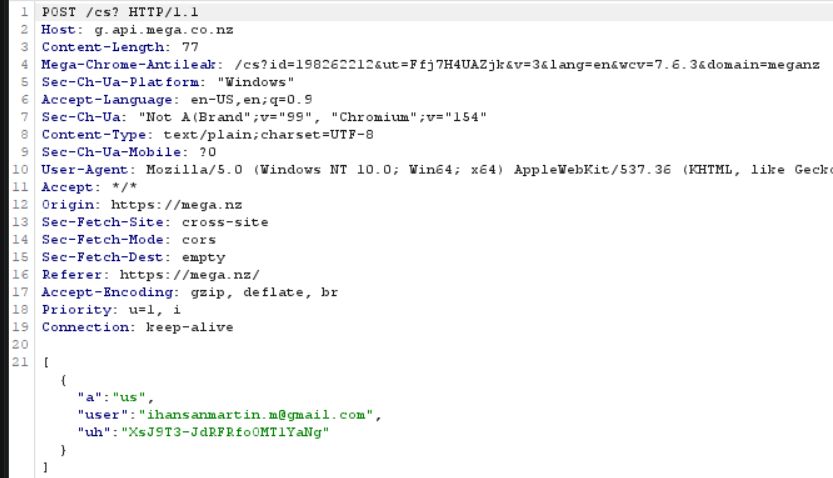
\includegraphics[width=0.9\textwidth]{peticionIntercep.png}
    \caption{Petición de login interceptada con BurpSuite}
\end{figure}

La figura 6 muestra la petición interceptada, la cual contiene campos de metadatos sobre el protocolo, versión del navegador, etc. Abajo del todo aparecen los datos de user y uh, que es ``XsJ9T3-JdRFRfoOMT1YaNg'' este es el hash correcto para iniciar sesión que necesitaremos más adelante.

A esta petición le llega la respuesta de parte del servidor con código 200 OK con algunos datos que se rescatan de la base de datos, como la master key ``k'', se puede ver en la figura 7.

\begin{figure}[H]
    \centering
    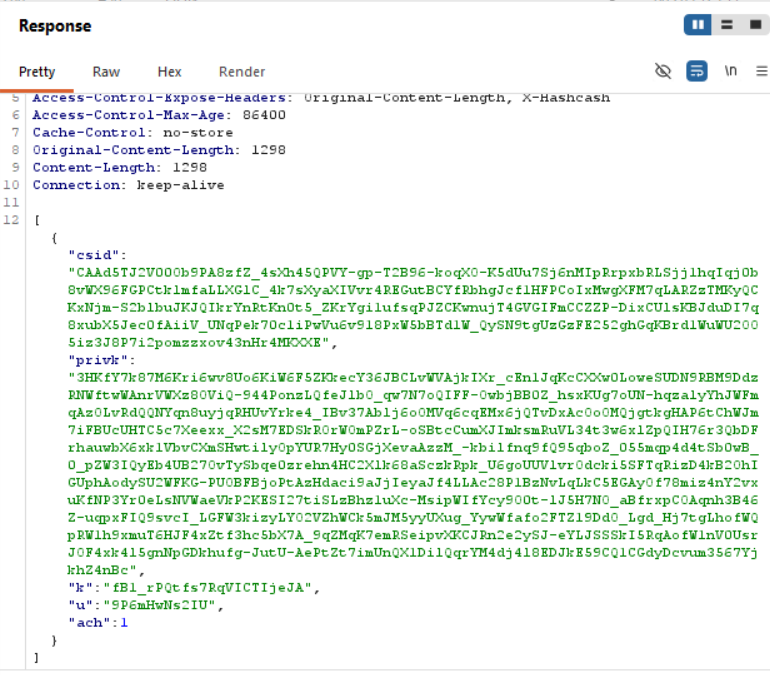
\includegraphics[width=0.9\textwidth]{responseIntercep.png}
    \caption{Respuesta de la petición de login interceptada con BurpSuite}
\end{figure}


\subsection{Realiza el intento de login}

Para esta parte se tuvo que interceptar un intento incorrecto de login, para luego modificar el campo uh con el hash correcto ya interceptado anteriormente.

\begin{figure}[H]
    \centering
    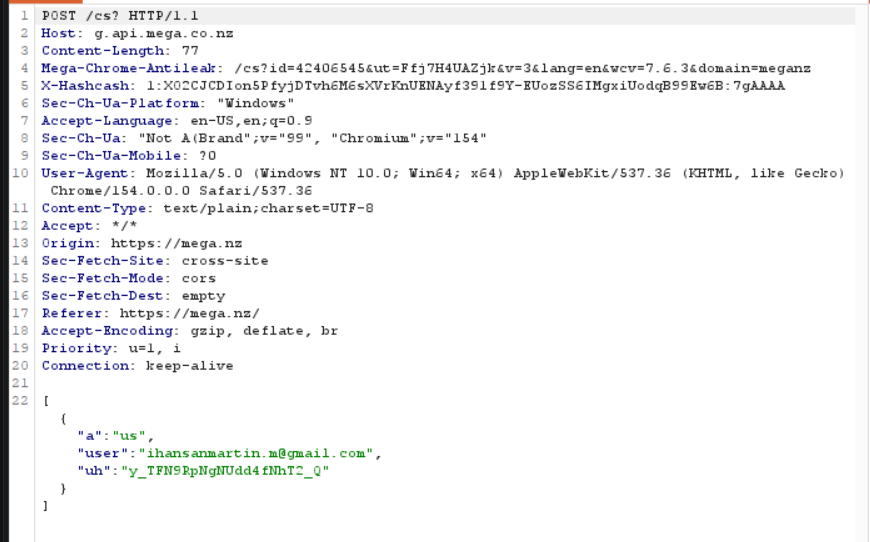
\includegraphics[width=0.9\textwidth]{peticionMala.png}
    \caption{Petición de login incorrecto.}
\end{figure}

En la figura 8 se puede observar un hash distinto al obtenido en el intento de login correcto interceptado, esto tiene como consecuencia directa una respuesta erronea de parte del servidor sin ningun dato de los que se veian en la figura 7, simplemente un arreglo con un único valor -9 que significa error de credenciales, como se puede ver en la figura 9.

\begin{figure}[H]
    \centering
    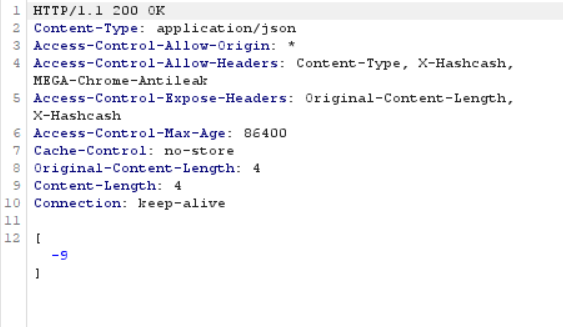
\includegraphics[width=0.9\textwidth]{responseMala.png}
    \caption{Respuesta de la petición de login incorrecto.}
\end{figure}

Para realizar el ataque \textbf{Pass The Hash} se debe enviar la petición incorrecta a la herramienta repeater de BurpSuite, y modificar el campo uh con el hash correcto.

\begin{figure}[H]
    \centering
    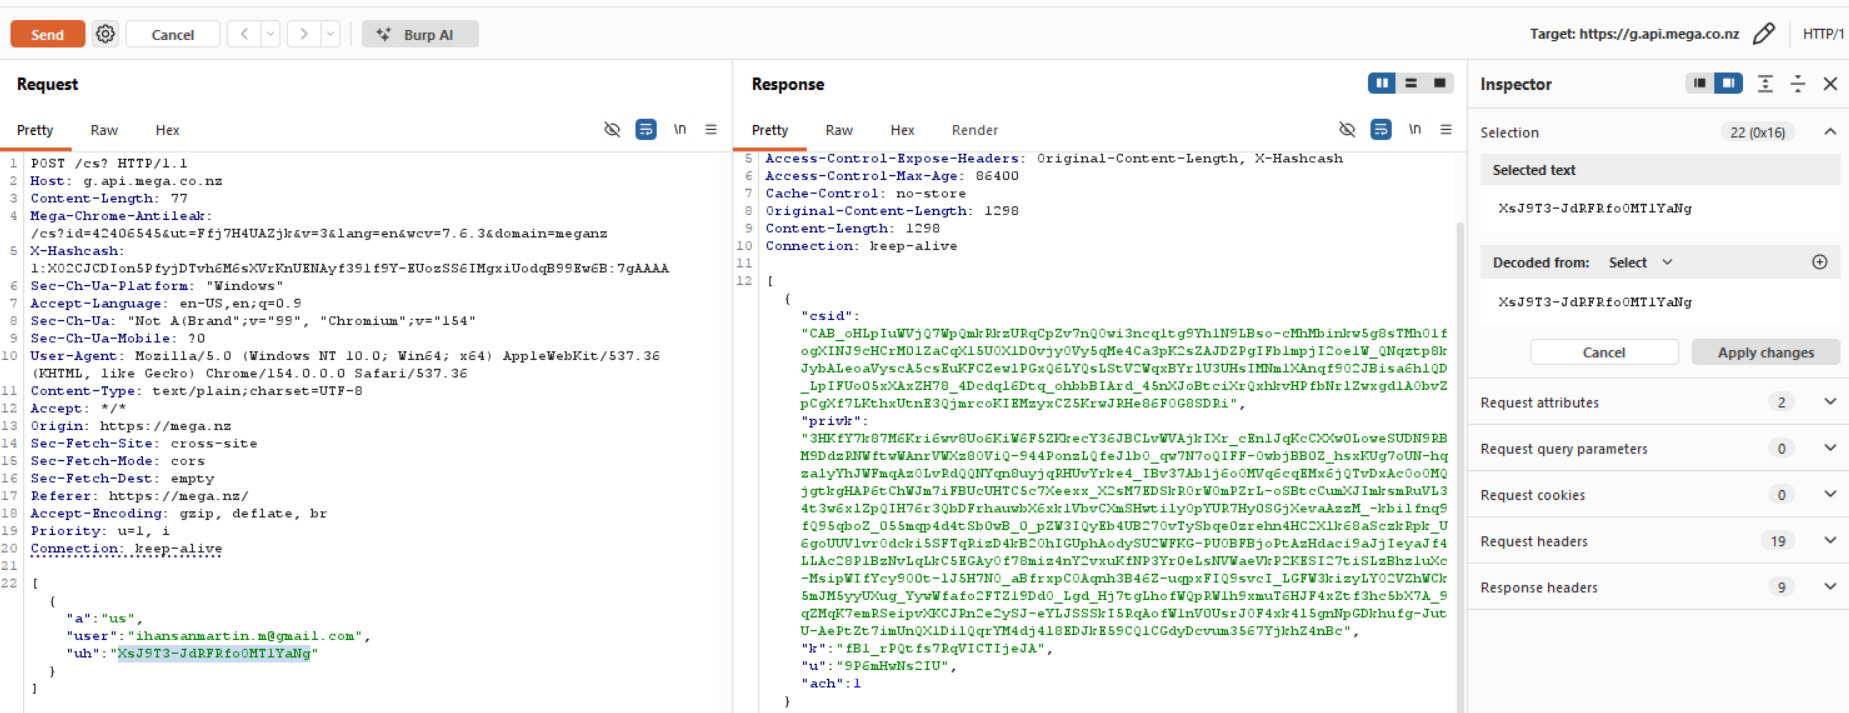
\includegraphics[width=1\textwidth]{pth.png}
    \caption{Ataque Pass The Hash realizado en repeater de BurpSuite.}
\end{figure}

En la figura 10 se puede ver el envío y respuesta de la petición modificado, dando como resultado la misma respuesta que se obtuvo en la figura 7, es decir, el ataque fue exitoso y se pudo iniciar sesión con el hash correcto sin necesidad de conocer la contraseña.

\subsection{Identifica las políticas de privacidad o seguridad}

\textbf{Seguridad:} \url{https://mega.io/security}

La arquitectura de seguridad de MEGA se basa en el principio de conocimiento cero, es decir, que los datos del usuario se cifran y descifran en el dispositivo de cada miembro de MEGA y no en sus servidores. Esto significa que ni siquiera la plataforma tiene acceso a los datos de sus usuarios. Además cuando alguien comparte un archivo a través de MEGA, el sistema usa la clave pública del destinatario para cifrar el contenido, el receptor utiliza su clave privada para descifrarlo localmente.

\textbf{Privacidad} \url{https://mega.io/privacy}

La política de privacidad de la plataforma está ligada directamente a su diseño de zero-knowledge, ellos no tendrán acceso a tus datos (data blindness), aunque esto no significa que no tomen tu dirección de correo electrónico, dirección IP, dispositivo, etc. para operar de manera correcta. Habrá veces que se necesite pedir permisos en el dispositivo para acceder a contactos, cámara, micrófono, etc. Por último, sus políticas se rigen por las regulaciones estrictas de protección de datos de la Unión Europea.

\subsection{Demuestra 4 conclusiones sobre la seguridad}

\begin{itemize}
    \item El uso de los algoritmos seleccionados en esta plataforma (PBKDF2 con HMAC-SHA512 y SHA-256) es adecuado para proteger las contraseñas de los usuarios y dificultar los ataques de fuerza bruta.
    \item La política zero-knowledge de MEGA garantiza que los datos del usuario estén seguros y privados en todo momento.
    \item El ataque de pass the hash demostró que a pesar de tener buena seguridad implementada a través del cliente, si un atacante logra interceptar el hash correcto, puede inciciar sesión sin necesidad de conocer la contraseña.
    \item Tanto el hashing de lado del cliente como de lado del servidor tienen sus pros y contras, todo dependerá de la implementación ya que ningún sistema se salva de vulnerabilidades, por lo que constantemente se debe estar revisando los mecanismos y estandares de seguridad.
\end{itemize}

% Please add the following required packages to your document preamble:
%\begin{table}[htbp]

\end{document}
